\documentclass{article}

% ============================================================
% MA 213 In-Class Worksheet Template
% Student-facing worksheet for lecture activities.
% ============================================================

\usepackage[margin=1in]{geometry}
\usepackage{amsmath}
\usepackage{xcolor}
\usepackage{parskip}
\usepackage{array}
\usepackage{enumitem}
\usepackage{booktabs}
\usepackage{graphicx}

\newcommand{\coursenumber}{MA 213}
\newcommand{\weekplaceholder}{6}
\newcommand{\lectureplaceholder}{15}
\newcommand{\lecturetitle}{What Would Happen If...? Think/Pair/Share}

\newcommand{\nameblank}{\rule{1.75in}{0.4pt}}
\newcommand{\idblank}{\rule{1.55in}{0.4pt}}
\newcommand{\shortblank}{\rule{1in}{0.4pt}}
\newcommand{\longblank}{\rule{0.93\linewidth}{0.4pt}}

\begin{document}

\begin{center}
  {\LARGE \coursenumber{} Week \weekplaceholder{}: Lecture \lectureplaceholder{}}\\
  {\large \lecturetitle{}}
\end{center}

\begin{enumerate}[label=\arabic*.,leftmargin=*,itemsep=.7em]
  \item \textbf{Your name:} \nameblank \hfill \textbf{BU ID:} \idblank
\end{enumerate}

\textbf{Big idea:} In the R demo, we generated a population with 88\% ``success.'' Then we took a random sample of size 1000, and computed the sample proportion. We repeated the sampling process many times and plotted a histogram of the sample proportions. The sampling distribution is shown below.

\begin{center}
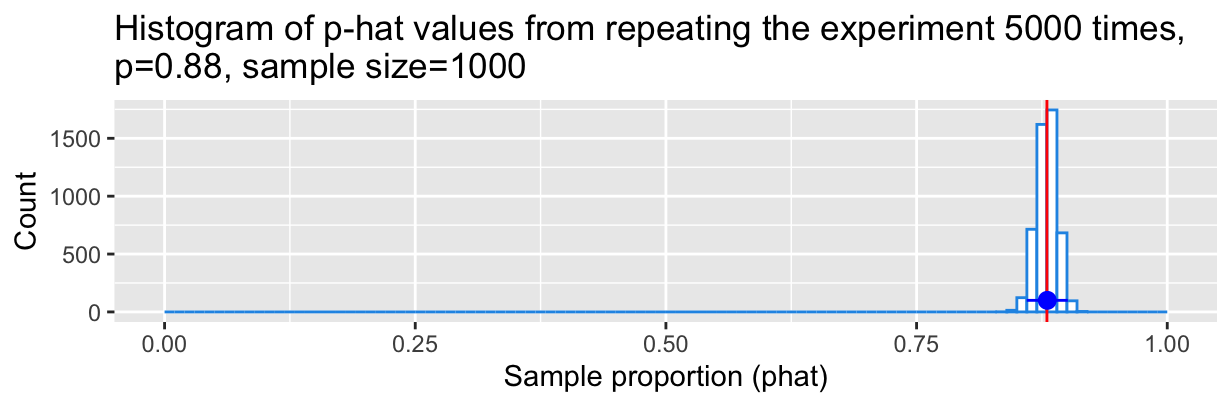
\includegraphics[width=0.6\textwidth]{sampling_distribution.png}
\end{center}

We'll come back to these predictions at the start of next lecture, so hang on to this sheet.

\section*{Step 1: Think (2 mins)}

\textbf{What if the population had 50\% success and the sample size were 100:}

\textbf{(a)} Where would you expect the middle of the sampling distribution to be? (write your answer as a decimal between 0 and 1)
\vspace{0.4in}

\textbf{(b)} Would the sampling distribution be symmetrical?
\vspace{0.4in}

\textbf{(c)} Would the sampling distribution be wider/narrower/the same (compared to the baseline above)?
\vspace{0.4in}

\textbf{What if the population had 99\% success and the sample size were 100:}

\textbf{(d)} Where would you expect the middle of the sampling distribution to be?
\vspace{0.4in}

\textbf{(e)} Would the sampling distribution be symmetrical?
\vspace{0.4in}

\textbf{(f)} Would the sampling distribution be wider/narrower/the same?
\vspace{0.4in}

\newpage
\section*{Step 2: Pair (2 mins)}

\begin{enumerate}[label=\arabic*.,leftmargin=*,itemsep=.7em, start=2]
  \item \textbf{Partner's name:} \nameblank \hfill \textbf{BU ID:} \idblank
\end{enumerate}

Compare your answers to (a)--(f) with your partner. Then work through this together:

\textbf{(g)} What would happen if the sample size were 10 (keeping $p=0.99$)? What would the sampling distribution of the sample proportion look like?
\vspace{0.6in}

\textbf{Our thoughts:}
\vfill

\end{document}
